\documentclass[sigconf,nonacm]{acmart}
\settopmatter{printacmref=false, printfolios=false}
\usepackage{tikz}
\usetikzlibrary{positioning,arrows.meta,calc}
% Placeholder for numbers we still have to measure. Remove before submitting.
\newcommand{\tbd}[1]{\textcolor{red}{[#1]}}

\begin{document}

\title{BridgeFinder: Finding People Across Structural Holes}

\author{Evan Lin and Eric Liu}
\email{{elin26, ericl8}@illinois.edu}
\affiliation{\institution{CS 470 project proposal, University of Illinois Urbana-Champaign}\country{}}

\begin{teaserfigure}
  \centering
  % Figure 1: the core flow as three minimal wireframe screens (grayscale).
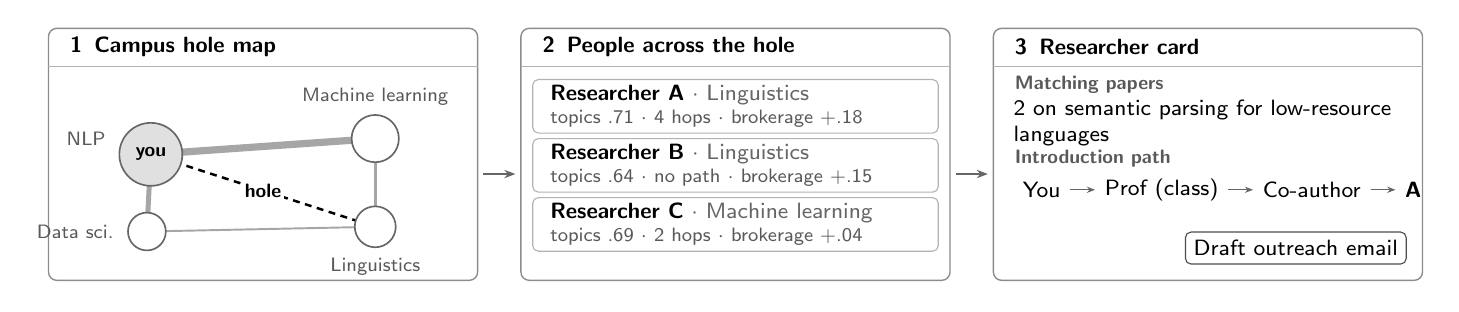
\begin{tikzpicture}[
    font=\sffamily\footnotesize,
    frame/.style={draw=black!45, line width=0.5pt, rounded corners=3pt},
    comm/.style={circle, draw=black!60, fill=white, line width=0.6pt},
    tie/.style={draw=black!35, line cap=round},
    small/.style={font=\sffamily\scriptsize, text=black!65},
  ]
  \def\W{5.45}\def\H{3.2}\def\G{0.55}\def\B{0.48}

  \foreach \i/\t in {0/{1\enspace Campus hole map}, 1/{2\enspace People across the hole}, 2/{3\enspace Researcher card}} {
    \pgfmathsetmacro\x{\i*(\W+\G)}
    \draw[frame] (\x,0) rectangle (\x+\W,\H);
    \draw[black!30] (\x,\H-\B) -- (\x+\W,\H-\B);
    \node[anchor=west, font=\sffamily\footnotesize\bfseries] at (\x+0.15,\H-\B/2) {\t};
  }
  \foreach \i in {0,1} {
    \pgfmathsetmacro\x{\i*(\W+\G)+\W}
    \draw[-{Stealth[length=4pt]}, line width=0.8pt, black!60] (\x+0.07,1.35) -- (\x+\G-0.07,1.35);
  }

  % Panel 1: communities and a structural hole.
  \coordinate (Y) at (1.3,1.6);  \coordinate (M) at (4.15,1.8);
  \coordinate (D) at (1.25,0.62); \coordinate (L) at (4.15,0.68);
  \draw[tie, line width=2.6pt] (Y) -- (M);
  \draw[tie, line width=1.8pt] (Y) -- (D);
  \draw[tie, line width=1pt] (M) -- (L);
  \draw[tie, line width=0.7pt] (D) -- (L);
  \draw[black, line width=0.9pt, dash pattern=on 2.5pt off 2pt] (Y) -- (L)
    node[pos=0.5, fill=white, inner sep=1pt, font=\sffamily\scriptsize\bfseries] {hole};
  \node[comm, fill=black!12, minimum size=0.8cm, font=\sffamily\scriptsize\bfseries] at (Y) {you};
  \node[comm, minimum size=0.6cm] at (M) {};
  \node[comm, minimum size=0.48cm] at (D) {};
  \node[comm, minimum size=0.52cm] at (L) {};
  \node[small, anchor=east] at ($(Y)+(-0.45,0.2)$) {NLP};
  \node[small, anchor=south] at ($(M)+(0,0.3)$) {Machine learning};
  \node[small, anchor=east] at ($(D)+(-0.3,0)$) {Data sci.};
  \node[small, anchor=north] at ($(L)+(0,-0.27)$) {Linguistics};

  % Panel 2: ranked researchers.
  \begin{scope}[shift={(\W+\G,0)}]
    \foreach \y/\name/\dept/\top/\hop/\gain in {
        1.95/Researcher A/Linguistics/.71/4 hops/+.18,
        1.2/Researcher B/Linguistics/.64/no path/+.15,
        0.45/Researcher C/Machine learning/.69/2 hops/+.04} {
      \draw[black!30, rounded corners=2pt] (0.15,\y-0.08) rectangle (\W-0.15,\y+0.6);
      \node[anchor=west] at (0.25,\y+0.4) {\textbf{\name} \textcolor{black!60}{$\cdot$ \dept}};
      \node[small, anchor=west] at (0.25,\y+0.1) {topics \top\ $\cdot$ \hop\ $\cdot$ brokerage \gain};
    }
  \end{scope}

  % Panel 3: researcher card.
  \begin{scope}[shift={(2*\W+2*\G,0)}]
    \node[small, anchor=west, font=\sffamily\scriptsize\bfseries] at (0.15,2.48) {Matching papers};
    \node[anchor=north west, text width=5cm, inner sep=0pt] at (0.25,2.3)
      {2 on semantic parsing for low-resource languages};
    \node[small, anchor=west, font=\sffamily\scriptsize\bfseries] at (0.15,1.55) {Introduction path};
    \node[anchor=west] (p0) at (0.25,1.15) {You};
    \node[right=9pt of p0] (p1) {Prof (class)};
    \node[right=9pt of p1] (p2) {Co-author};
    \node[right=9pt of p2] (p3) {\textbf{A}};
    \foreach \a/\b in {p0/p1, p1/p2, p2/p3} \draw[-{Stealth[length=3pt]}, black!60] (\a) -- (\b);
    \node[draw=black!70, rounded corners=2pt, inner sep=3pt, anchor=south east] at (\W-0.2,0.2)
      {Draft outreach email};
  \end{scope}
\end{tikzpicture}

  \caption{Core flow. (1) UIUC co-authorship communities; dashed = a structural hole (similar topics, almost
  no joint papers). (2) Researchers across the hole, ranked. (3) Their matching papers and an introduction path.}
  \label{fig:flow}
\end{teaserfigure}

\maketitle

\section{Objective}
When students search for a research mentor or researchers seek collaborators, they tend to search through connections they know: their lab, their department, etc. However, novel information spreads through weak ties~\cite{granovetter1973}, and individuals spanning structural holes between disconnected communities will be more likely to generate innovative ideas~\cite{burt2004}. Interdisciplinary research often harbors these exact structural holes. At UIUC and other universities, separate groups frequently tackle similar problems for years without co-authoring a single paper.  \textbf{BridgeFinder} finds these gaps in the co-authorship graph and names the people on the other side. 

\section{Related Work}
Current tools like Illinois Experts~\cite{experts} and Google Scholar will match by keyword, but fail to consider graph topology, treating researchers like isolated documents. LinkedIn's ``People You May Know'' and link prediction~\cite{libennowell2007} favor triadic closure, which reinforces mutual connections instead of brokerage. \textbf{BridgeFinder} explicitly detects structural holes to recommend collaborators across disconnected communities.


\section{Course Concepts \& Network Analysis}
Our project centers on \textbf{brokerage} (Lesson~1): weak ties that act like local bridges, passing information between two disconnected groups. We will build a graph where the nodes are UIUC researchers in OpenAlex~\cite{openalex} and the edges are co-authorships, weighted by the number of joint papers; each node is tagged with its OpenAlex topics. Louvain modularity (Lesson~10) splits the graph into research communities, and a \emph{hole} is two communities with similar topics but few joint papers. For a student, we rank researchers at least three steps away by cosine similarity of OpenAlex topic profiles, boosted by the number of introduction paths to them.

\emph{Alternatives from class:} triadic closure only finds people who are already nearby; Girvan--Newman could not split even a 150-node graph in 148\,s in our pilot, so we use Louvain.

\emph{Claim that could be false:} among researchers three or more steps away, our ranking will place people's real 2020--24 new collaborators in its top 10 more often than topic similarity alone. A pilot found only a small, uncertain gain, so this may not hold.

\section{Proposed Work}
We will create a web app with at least the three screens shown in Figure~\ref{fig:flow}. A student will be able to pick the professors whose classes they liked. The app will then show the campus map (derived from joint papers in OpenAlex). The app will also display a ranked list of researchers in other research communities, and, for each one, the papers that match their interests and who could introduce them. To create the campus map, we will write a Python program to preprocess the UIUC co-authorship graph from OpenAlex (around 110,000 papers from 2015 to 2024).

\noindent\textbf{By Oct 30: } We will have the preprocessed graph and communities, as well as the first version of the app, and feedback from round 1. 

\noindent\textbf{By mid-Nov: } We will have the researcher cards, introduction paths, and the round 2 feedback. 

\noindent\textbf{By Dec 9: } We will polish the app based on feedback, and record the final evaluation and video. 

\noindent\textbf{Assumptions: } We assume the following: the co-authors of papers know each other; OpenAlex correctly identifies people; the OpenAlex topics correctly capture what a researcher worked on; professors who teach a class do research in the corresponding area. Finally, a disclaimer is that the app can't actually tell if a professor is taking students, so it should just be used as a suggestion about people to talk to.

\section{Preliminary Design}
The core flow of the app follows Figure~\ref{fig:flow}. The student first picks the professors from classes they enjoyed. Then, the map will show their research communities and holes between them. Beside this, the app will also display a ranked list of researchers across those holes, and each of the researchers can be clicked to open a researcher card that shows their matching papers and the introduction path. Unlike previous work such as Illinois Experts or Google Scholar, which all start with a search box, we collect the user's interests, then show the map first so users can see where the gaps are as well as the overall research landscape. Additionally, we provide reasoning for each suggestion.

\section{Users}
Our target user group is UIUC students who liked a class and want to do research in the topic the class covered. A student will be attached to the graph through the professors whose class they enjoyed, and the app will be able to find researchers with similar work (but outside of the professors' circles) along with who could introduce them. We will try to recruit around 10 people (friends and classmates) to test the app through each of the rounds. 

\section{Evaluation}

(1)~\textbf{Backtest:} Looking at the data from 2015 to 2019, we will predict the top 10 relevant people for each researcher using different methods (our method, triadic closure, topic only). We then count how often those people include someone who they actually started working with in 2020 to 2024.

\noindent(2)~\textbf{Blind rating: } We will give each participant around 15 researcher cards (name, department, recent papers), five from each method (our method, triadic closure, topic only). These will be shuffled so they don't know which method produced them. We can then have them rate each researcher based on relevance of their work to their interests, and whether they knew the person already. Our method succeeds if more of its cards are both relevant and new to the participant.

\noindent(3)~\textbf{Usefulness: } We will also survey if our users would feel comfortable enough to contact the suggested people.

\noindent\emph{AI Use:} We used Claude as a collaborator to brainstorm ideas, and create an initial draft. Everything was reviewed and verified. 

\bibliographystyle{ACM-Reference-Format}
\bibliography{references}
\end{document}
